% latex.tex
\PassOptionsToPackage{usenames,dvipsnames}{xcolor}
\documentclass{beamer}
\usetheme[hideothersubsections,height=6mm]{Berkeley}
\setbeamertemplate{navigation symbols}{}

\usepackage{listings}
\usepackage{hyperref}
\usepackage{tikz}
\usepackage{graphicx}

\usetikzlibrary{arrows,automata}

\definecolor{MyDarkGreen}{rgb}{0.0,0.4,0.0}

% For faster processing, load LaTeX syntax for listings
\lstloadlanguages{[LaTeX]TeX}%
\lstset{language=[LaTeX]TeX, frame=single, basicstyle=\small\ttfamily,
  keywordstyle=[1]\color{Blue}\bf, keywordstyle=[2]\color{Purple},
  keywordstyle=[3]\color{Blue}\underbar, identifierstyle=,
  commentstyle=\usefont{T1}{pcr}{m}{sl}\color{MyDarkGreen}\small,
  stringstyle=\color{Purple}, showstringspaces=false, tabsize=5,
  % Put standard LaTeX macros not included in the default
  % language here
  morekeywords={},
  % Put LaTeX macro parameters here
  morekeywords=[2]{},
  % Put user defined macros here
  morekeywords=[3]{}, morecomment=[l][\color{Blue}]{...},
  numbers=left, firstnumber=1, numberstyle=\tiny\color{Blue},
  stepnumber=5 }

\title{\LaTeX}
\subtitle{Create Snazzy Documents}
\author{Chris Sims \\ chris@jcsi.ms}
\date{24 Sep 2013}

\begin{document}
\lstset{language=[LaTeX]TeX}
\frame{\titlepage}

\begin{frame}{Outline}
  \tableofcontents
\end{frame}


% -------------Why?------------%
\section{Why \LaTeX?}
\begin{frame}
  \frametitle{What Is It?}
  \begin{itemize}
  \item pronounced either lay-tech or lah-tech
  \item a set of macros on top of \TeX, a markup and programming
    language originally created by Donald Knuth
  \item a language designed to let the writer focus on content, while
    taking care of layout
  \end{itemize}
\end{frame}

\begin{frame}
  \frametitle{Uh...Why Can't I Just Type What I Want?}

  \begin{itemize}
  \item consistent and professional typography
  \item fully customizable and extendable
  \item no special file formats
  \item vast amount of packages available for almost any application
  \end{itemize}

\end{frame}

\section{Getting Started}
\begin{frame}
  \frametitle{Installation}
  Various incarnations of the TeXLive package are available:
  \begin{itemize}
  \item typically available in Linux package managers
  \item MacTex package for OSX
  \item MikTeX for Windows
  \end{itemize}
  Editor support is widely available:
  \begin{itemize}
  \item vim -
    \href{http://github.com/gerw/vim-latex-suite}{vim-latex-suite}
  \item emacs -
    \href{https://www.gnu.org/software/auctex/}{auctex}
  \item sublime text - \href{https://github.com/SublimeText/LaTeXTools}{{\LaTeX}Tools}
  \item a large number of dedicated editors for {\LaTeX}
  \end{itemize}
\end{frame}

\begin{frame}[fragile]
  \frametitle{Basics}
  A simple ``Hello World'' example:
\begin{lstlisting}
\documentclass{article}

\begin{document}
Hello world!
\end{document}
\end{lstlisting}
\end{frame}

\section{Graphics}
\begin{frame}
  \frametitle{Finite Automata}

  \begin{center}
    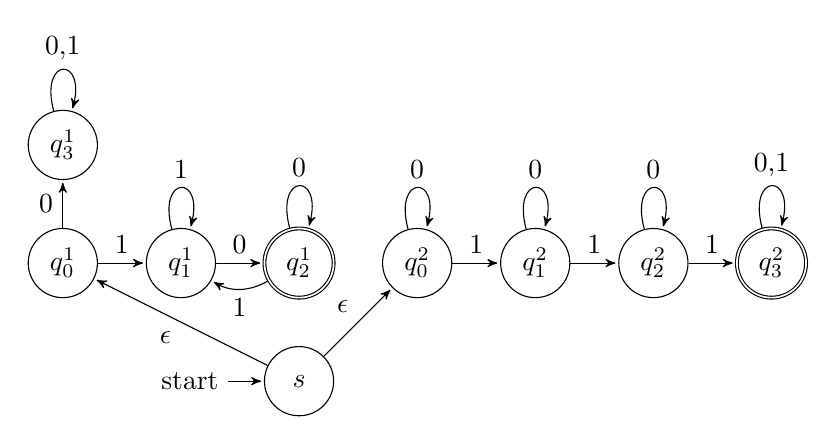
\begin{tikzpicture}[>=stealth',shorten >=1pt,auto,node distance=1.5cm]
      %% FA from 1a
      \node[state]            (q10)                       {$q^1_0$};
      \node[state]            (q11) [right of=q10]        {$q^1_1$};
      \node[state, accepting] (q12) [right of=q11]        {$q^1_2$};
      \node[state]            (q13) [above of=q10]        {$q^1_3$};

      \path[->]  (q10) edge              node {1} (q11);
      \path[->]  (q11) edge [loop above] node {1} (q11);
      \path[->]  (q11) edge              node {0} (q12);
      \path[->]  (q12) edge [loop above] node {0} (q12);
      \path[->]  (q12) edge [bend left]  node {1} (q11);
      \path[->]  (q10) edge              node {0} (q13);
      \path[->]  (q13) edge [loop above] node {0,1} (q13);

      %%%%%%%%%%%%%%%%%%%%%%%%%%%%%%%%%%%%%%%%%%%%%%%%%%%%%%%%%%% 
      %% FA from 1b
      %%%%%%%%%%%%%%%%%%%%%%%%%%%%%%%%%%%%%%%%%%%%%%%%%%%%%%%%%%% 
      \node[state]            (q20) [right of=q12]       {$q^2_0$};
      \node[state]            (q21) [right of=q20]       {$q^2_1$};
      \node[state]            (q22) [right of=q21]       {$q^2_2$};
      \node[state, accepting] (q23) [right of=q22]       {$q^2_3$};


      \path[->]  (q20) edge              node {1} (q21);
      \path[->]  (q20) edge [loop above] node {0} (q20);
      \path[->]  (q21) edge              node {1} (q22);
      \path[->]  (q21) edge [loop above] node {0} (q21);
      \path[->]  (q22) edge              node {1} (q23);
      \path[->]  (q22) edge [loop above] node {0} (q22);
      \path[->]  (q23) edge [loop above] node {0,1} (q23);

      %%%%%%%%%%%%%%%%%%%%%%%%%%%%%%%%%%%%%%%%%%%%%%%%%%%%%%%%%% 
      %% Encompassing NFA
      \node[state, initial]   (s) [below of=q12]   {$s$};

      \path[->]  (s) edge node {$\epsilon$} (q10);
      \path[->]  (s) edge node {$\epsilon$} (q20);
    \end{tikzpicture}
  \end{center}
  \begin{block}{Packages}
    The \texttt{tikz} package and \texttt{automata} and \texttt{arrows
      tikz} libraries are required for this.
  \end{block}
\end{frame}
\begin{frame}
  \frametitle{Images}
  \begin{center}
    \includegraphics[scale=0.5]{chick}
  \end{center}
  \begin{block}{Packages}
    The \texttt{graphicx} package is required to import images.
  \end{block}
\end{frame}
\section{Mathematics}
\begin{frame}
  \frametitle{Math Environments}
  There are two main methods of inserting mathematical statements into
  your text:
  \begin{itemize}
  \item inline: \texttt{\$<maths>\$}
  \item the math environment: \texttt{\textbackslash [ maths
      \textbackslash]}
  \end{itemize}
  There are a handful of specialized math environments which can come
  in handy:
  \begin{itemize}
  \item \texttt{align} and \texttt{align*} - align each line on
    arbitrary characters (e.g. the equals sign)
  \item \texttt{proof} - a bit of extra formatting typically seen in proofs
  \end{itemize}
  \begin{block}{Not Your Average Environment}
    Many things are different in the math environments, so make sure
    to read through the Mathematics and Advanced Mathematics
    sections in the WikiBook
  \end{block}
\end{frame}
\section{Tables}
\begin{frame}[shrink]
  \frametitle{Basic Tables}

  \begin{table}[h]
    \centering

    \begin{tabular}{l l c r r c}
      ID & Kernel & Degree & $\gamma$ & Cost & Cross-Validated Error (\%) \\
      \hline
      1  & Linear         &   &        & 0.01 & 20.8 \\
      2  & Linear         &   &        & 0.1  & 22.1 \\
      3  & Polynomial     & 2 &        & 0.01 & 40.0 \\
      4  & Polynomial     & 2 &        & 0.1  & 34.8 \\
      5  & Polynomial     & 2 &        & 1    & 19.4 \\
      6  & Polynomial     & 2 &        & 10   & 18.1 \\
      7  & Polynomial     & 2 &        & 100  & 19.3 \\
      8  & Polynomial     & 3 &        & 1    & 18.7 \\
      9  & Radial         &   & 0.125  & 1    & 18.3 \\
      10 & Radial         &   & 0.125  & 10   & 19.0 \\
      11 & Radial         &   & 0.1    & 1    & 18.0 \\
      12 & Radial         &   & 0.05   & 1    & 19.0 \\
      13 & Radial (tuned) &   & 0.0625 & 8    & 16.8 \\
      \hline
    \end{tabular}
    \caption{Results from model search}
  \end{table}
\end{frame}
\begin{frame}[fragile,shrink]
  \frametitle{Basic Tables, ctd}
  \begin{center}
\begin{lstlisting}[frame=none]
\begin{table}[h]
  \centering

  \begin{tabular}{l l c r r c}
    ID & Kernel & Degree & $\gamma$ & Cost &
    Cross-Validated Error (\%) \\
    \hline
    1  & Linear         &   &        & 0.01 & 20.8 \\
    2  & Linear         &   &        & 0.1  & 22.1 \\
    3  & Polynomial     & 2 &        & 0.01 & 40.0 \\
    4  & Polynomial     & 2 &        & 0.1  & 34.8 \\
    5  & Polynomial     & 2 &        & 1    & 19.4 \\
    6  & Polynomial     & 2 &        & 10   & 18.1 \\
    7  & Polynomial     & 2 &        & 100  & 19.3 \\
    8  & Polynomial     & 3 &        & 1    & 18.7 \\
    9  & Radial         &   & 0.125  & 1    & 18.3 \\
    10 & Radial         &   & 0.125  & 10   & 19.0 \\
    11 & Radial         &   & 0.1    & 1    & 18.0 \\
    12 & Radial         &   & 0.05   & 1    & 19.0 \\
    13 & Radial (tuned) &   & 0.0625 & 8    & 16.8 \\
    \hline
  \end{tabular}
  \caption{Results from model search}
\end{table}
\end{lstlisting}
  \end{center}
\end{frame}
\section{Code Listings}
\begin{frame}[fragile]
  \frametitle{Code Listings}
  Code listings are used to display source code in a document.
  \begin{itemize}
  \item \texttt{lstlisting} - listing environment
  \item many options available to customize and designate language
  \end{itemize}
  \begin{block}{Package Required}
    The \texttt{listings} package is required to use code listings.
  \end{block}
\end{frame}
\section{Making {\LaTeX} Your Own}

\begin{frame}
  \frametitle{Macros}
  There are a handful of commands to abstract some common routines
  \begin{itemize}
  \item \texttt{newcommand} - takes a name, num of arguments, and a
    definition
  \item \texttt{newenvironment} - takes a name, num of arguments, and
    \texttt{begin} and \texttt{end} blocks
  \item basic programming constructs like conditionals and loops are
    also available to use
  \end{itemize}
\end{frame}
\section{Help!}
\begin{frame}
  \frametitle{Getting Help}
  {\LaTeX} is crazy complicated - where do you even start?
  \begin{itemize}
  \item \href{http://en.wikibooks.org/wiki/LaTeX}{{\LaTeX} WikiBook}:
    not exhaustive, but a great source
  \item \href{http://tex.stackexchange.com}{\TeX.stackexchange.com}:
    like StackOverflow, but for {\TeX}
  \item packages have documentation on \href{http://www.ctan.org}{CTAN (Comprehensive {\TeX}
      Archive Network)}
  \item examples are a great place to find snippets (like this document!)
  \item ask me!
  \end{itemize}
\end{frame}
\end{document}
